\newpage
\section{Schaltanlagen / Umspannwerke}

\subsection{Aufgabe}

\begin{itemize}
    \item Stromfluss herstellen oder unterbrechen
    \item Betriebsmittel unter Spannung setzen oder spannungslos schalten
    \item Topologie ändern
    \item Strom- und Spannungsmessung
\end{itemize}

\subsection{Aufbau}

\begin{center}
    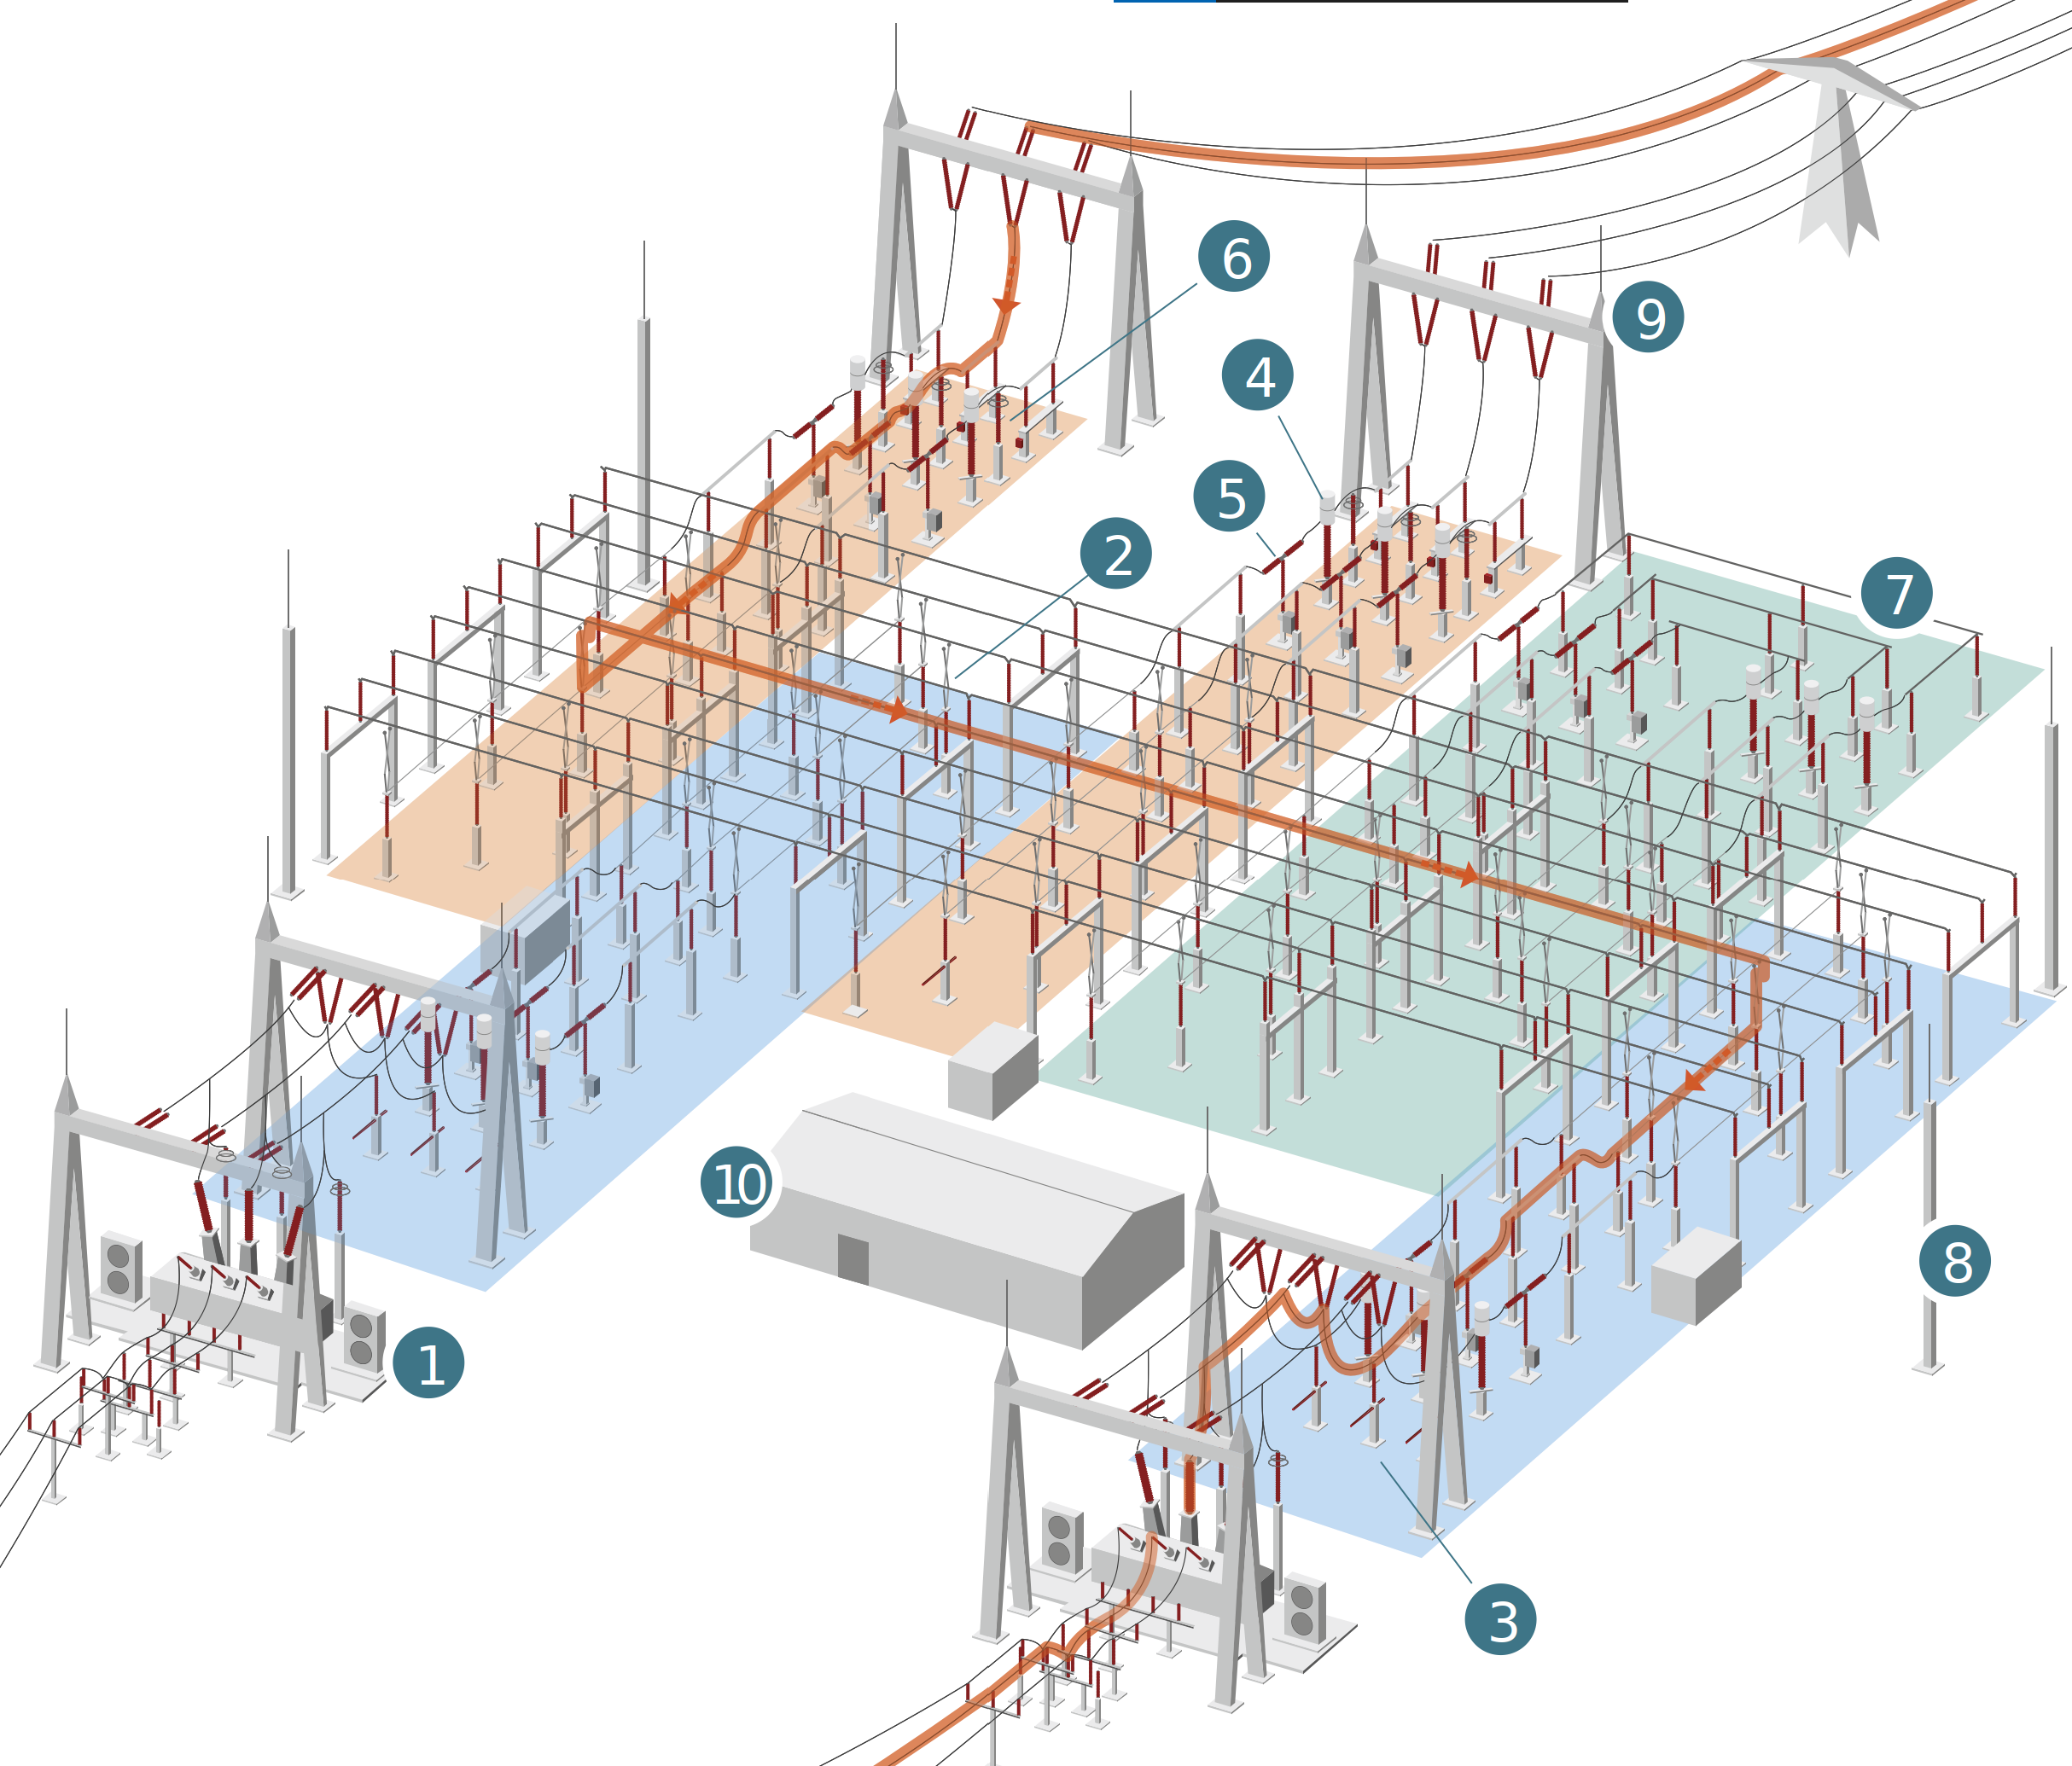
\includegraphics[width=0.98\columnwidth]{images/Aufbau_Schaltanlagen_1.png}
\end{center}

\begin{enumerate}
    \item Transformatoren
    \item Trennschalter
    \item Erdungsschalter
    \item Strom- und Spannungswandler
    \item Leistungsschalter
    \item Überspannungsableiter
    \item Sammelschiene
    \item Blitzschutzmast
    \item Portal
    \item Relais- und Betriebsgebäude
\end{enumerate}


\subsection{Transformator}

\begin{itemize}
    \item Veränderung der Spannung
    \item Öl zur Isolation und zum Wärmeabtransport
\end{itemize}

\begin{minipage}[c]{0.58\columnwidth}
    \begin{center}
        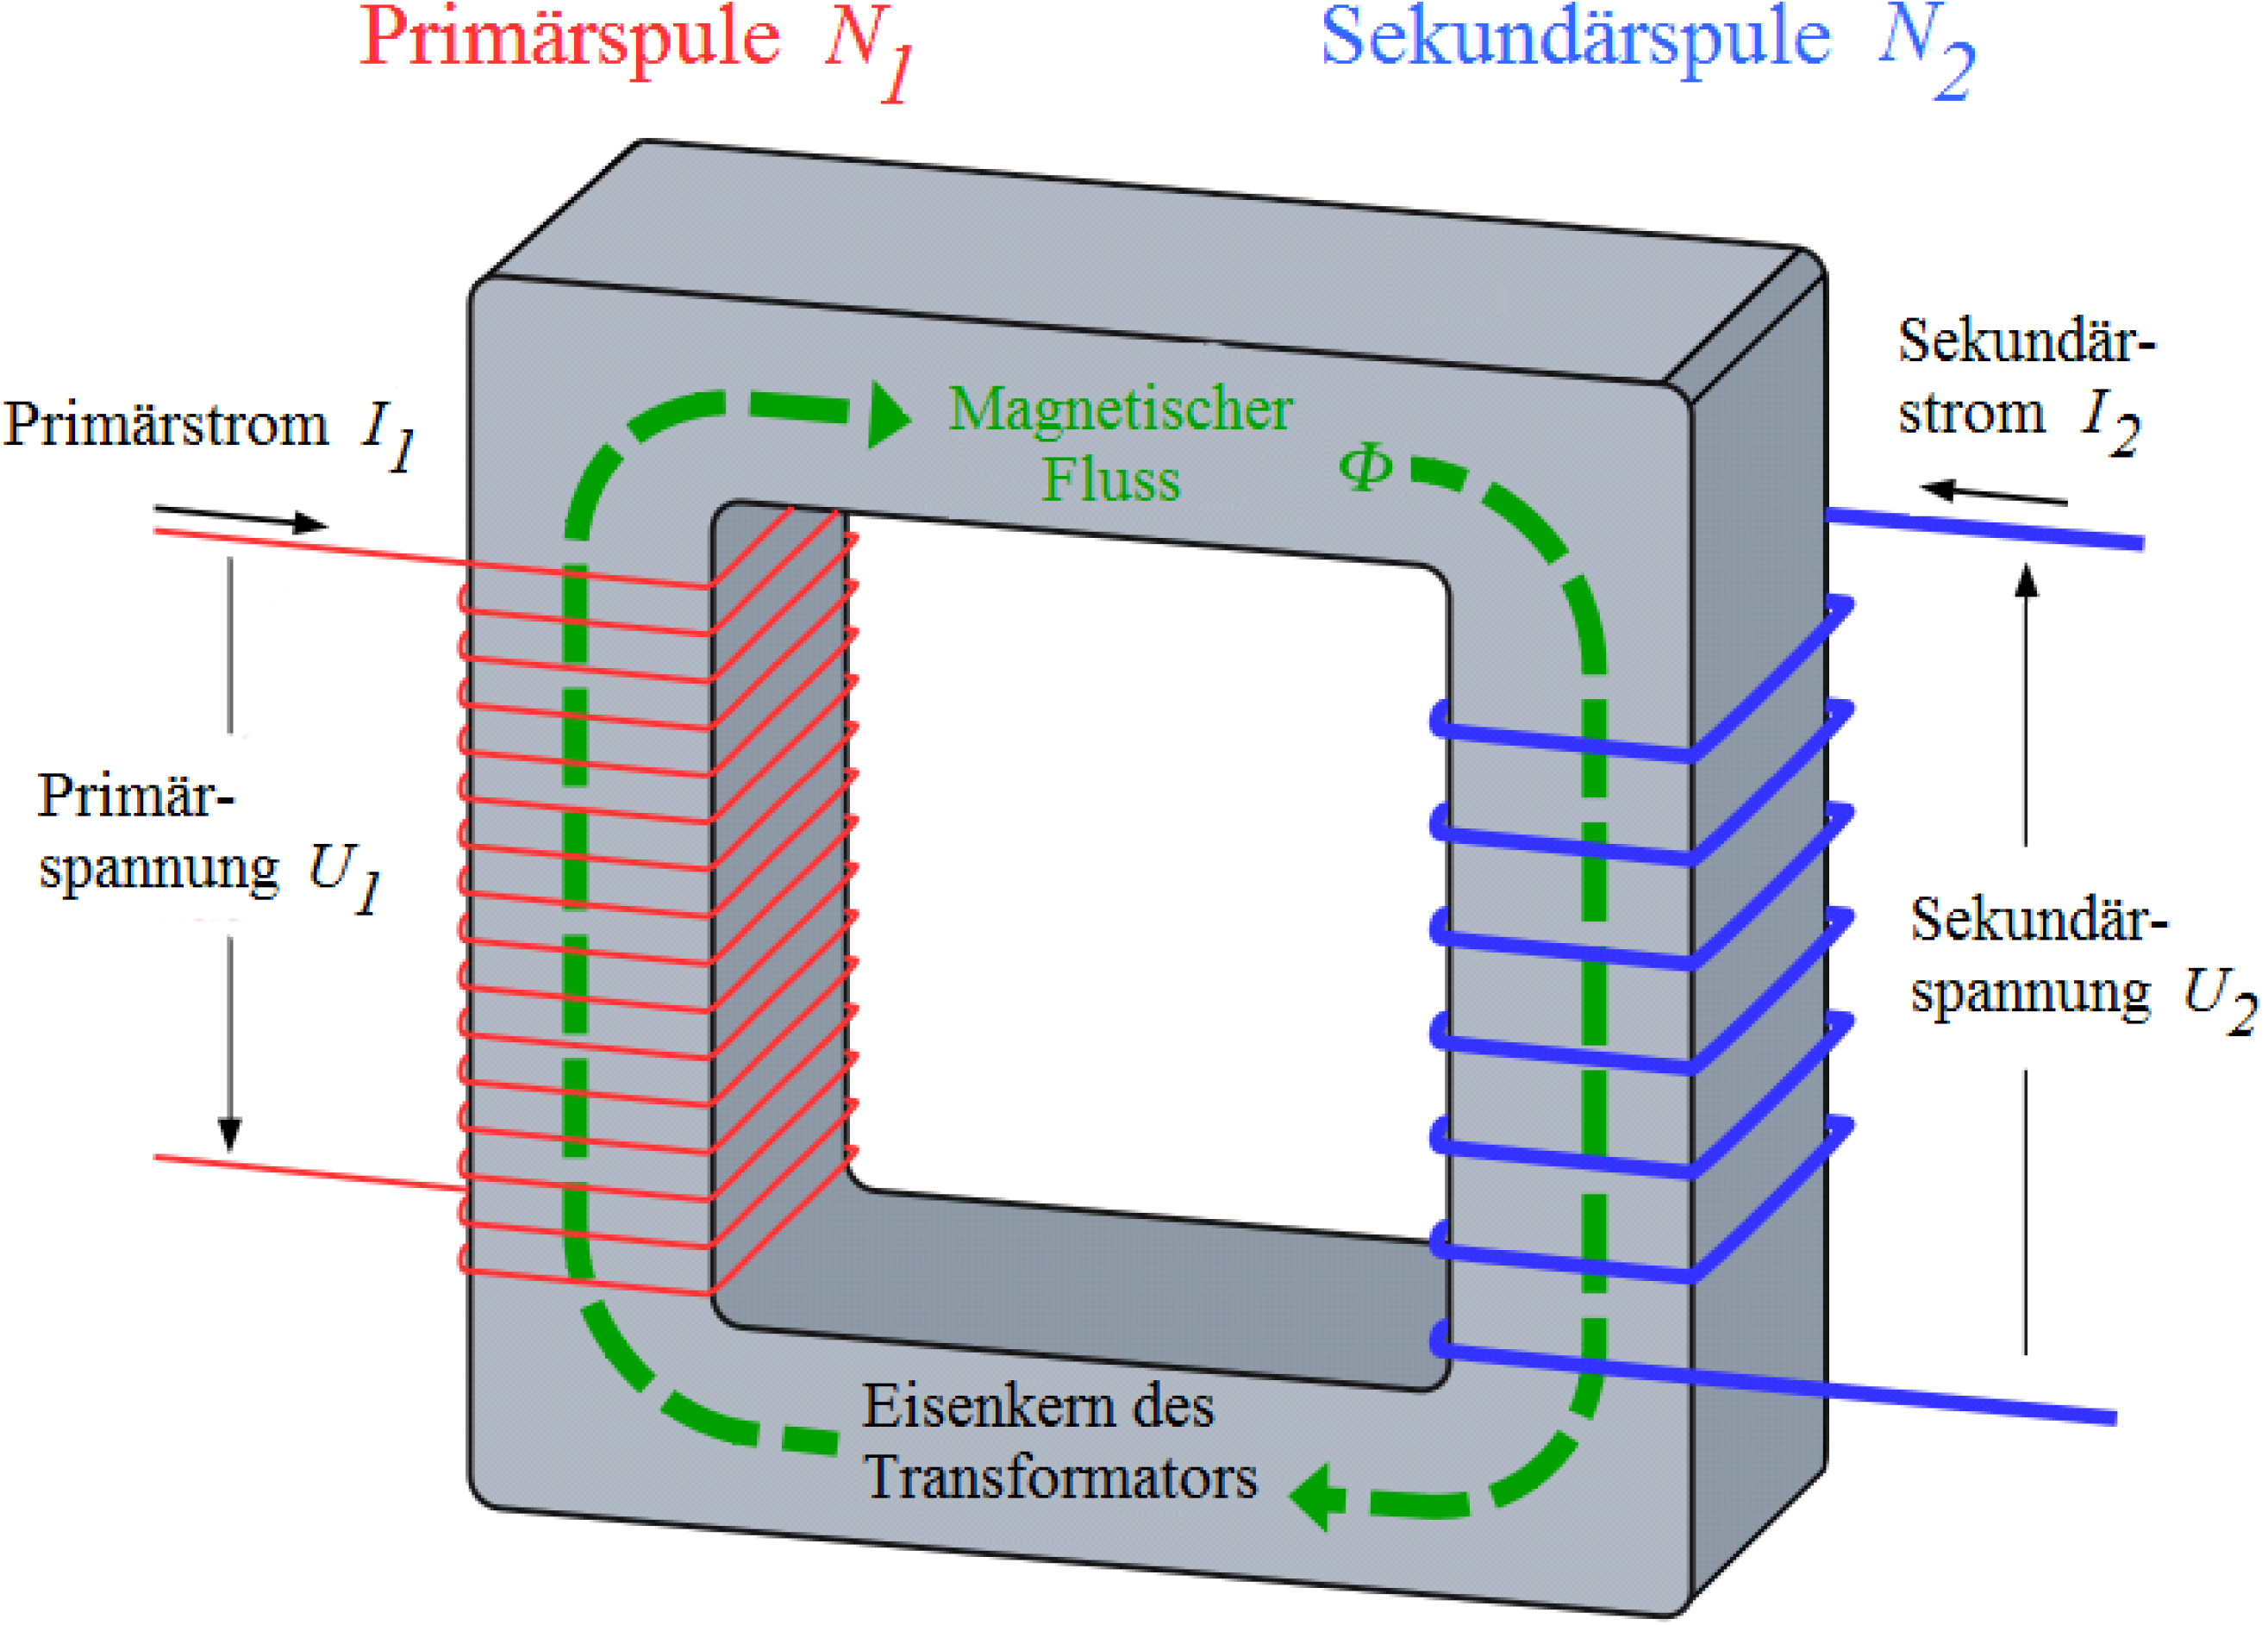
\includegraphics[width=0.98\textwidth, align=c]{images/Transformator_1.png}
    \end{center}
\end{minipage}
\hfill
\begin{minipage}[c]{0.38\columnwidth}
    \begin{center}
        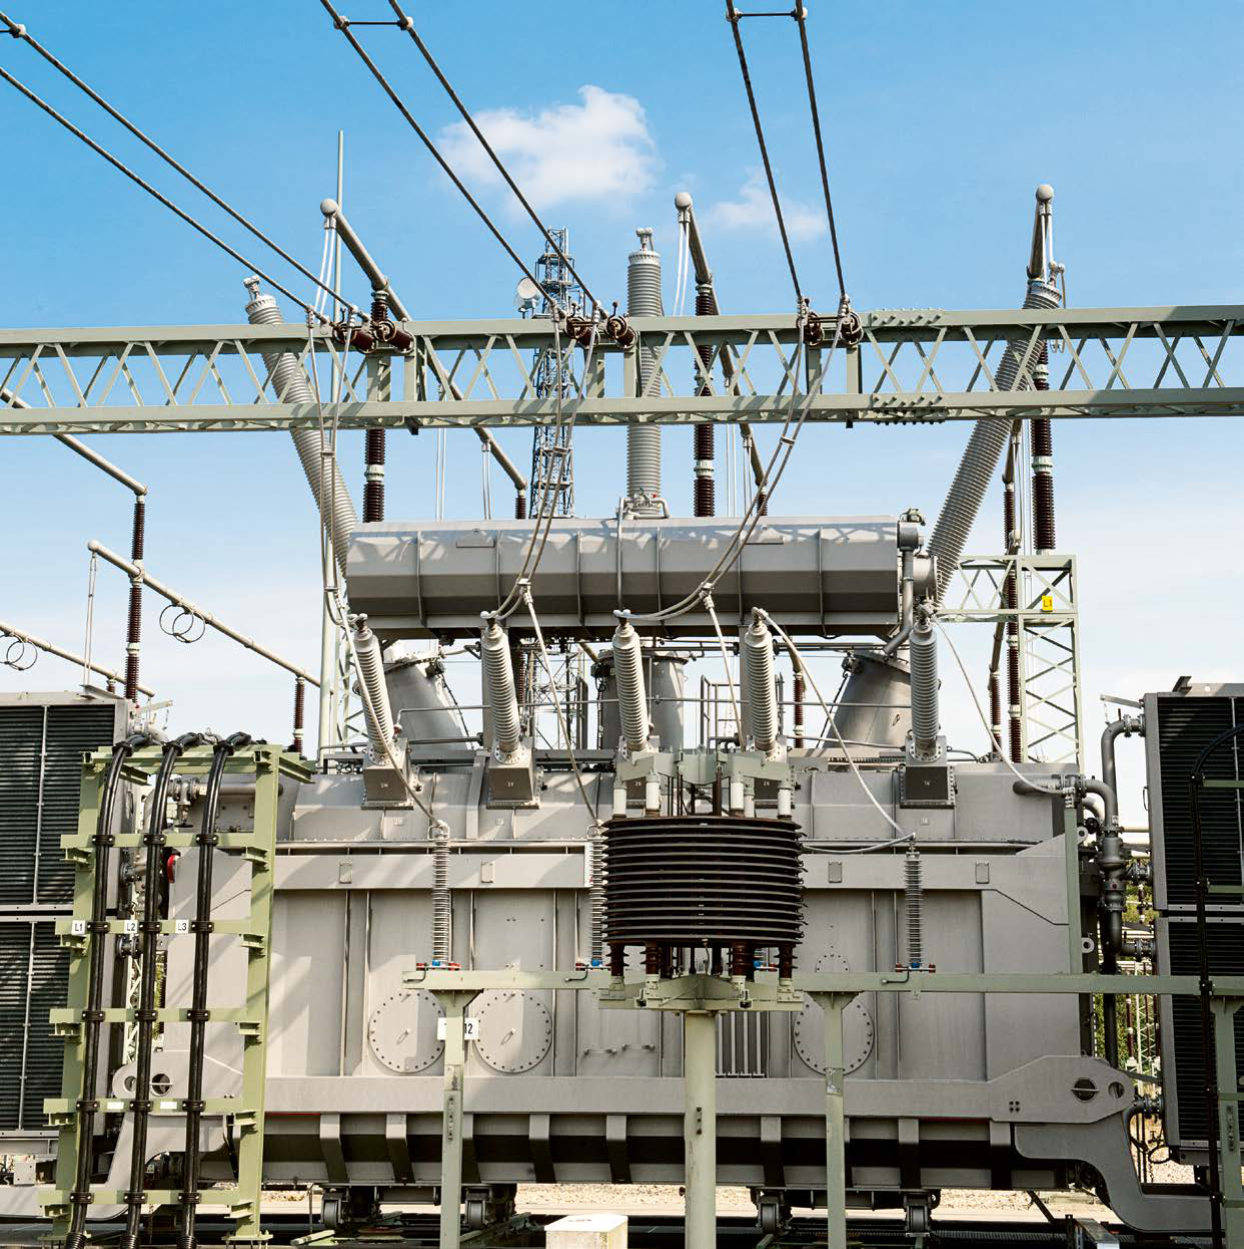
\includegraphics[width=0.98\textwidth, align=c]{images/Transformator_2.png}
    \end{center}
\end{minipage}


\subsection{Leistungsschalter}



\begin{minipage}[c]{0.28\columnwidth}
    \begin{center}
        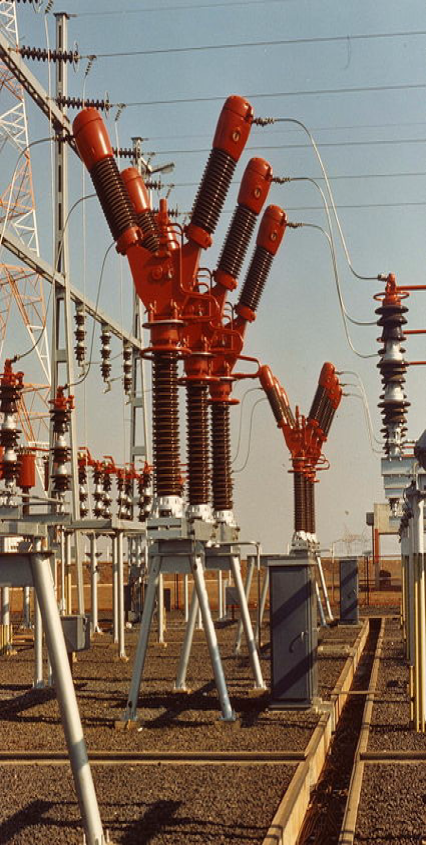
\includegraphics[width=0.98\textwidth, align=c]{images/Leistungsschalter.png}
    \end{center}
    
\end{minipage}
\hfill
\begin{minipage}[t]{0.68\columnwidth}
    \begin{itemize}
        \item Schaltet \textbf{Strom}
        \item Ein- und Ausschalten von Leitungen und Anlagenteile
        \item Schaltet im Normalbetrieb und im Fehlerfall\\(Kurzschlussstromunterbrechung)
    \end{itemize}
\end{minipage}


\subsection{Lastschalter}

\begin{itemize}
    \item Schaltet \textbf{Strom}
    \item Kann bis zu ca. 2-fachem Laststrom unterbrechen
\end{itemize}


\subsection{Trennschalter}

\begin{minipage}[c]{0.5\columnwidth}
    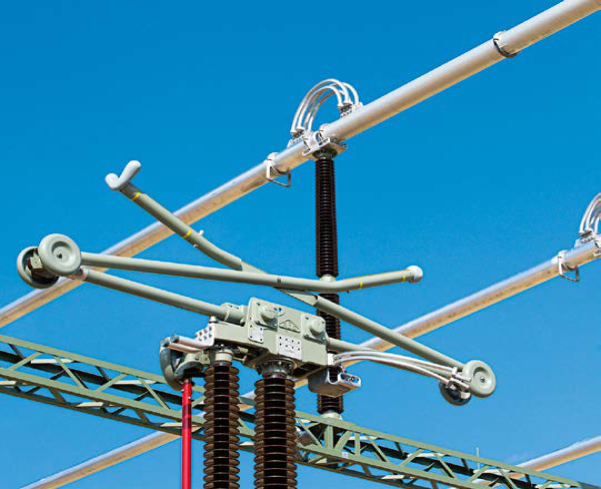
\includegraphics[width=0.98\textwidth]{images/Trennschalter.png}    
\end{minipage}

\begin{itemize}
    \item Leitungs- oder Sammelschienentrennschalter
    \item öffnen eines Stromkreises (Trennung einer Anlage von den restlichen Anlagen)
    \item Die Trennschalter schalten \textbf{keinen Strom}.
\end{itemize}


\subsection{Sonstiges}

\begin{minipage}[c]{0.48\columnwidth}
    \subsubsection{Messwandler}
\end{minipage}
\hfill
\begin{minipage}[c]{0.48\columnwidth}
    \subsubsection{Überspannungsableiter}
\end{minipage}

\begin{minipage}[c]{0.48\columnwidth}
    Messung der Spannung und Strom für Erkennung des Betriebszustandes
\end{minipage}
\hfill
\begin{minipage}[c]{0.48\columnwidth}
    Spannungsabhängiger Widerstand, Bei hoher Spannung verringert sich Widerstand schlagartig
\end{minipage}

\vspace{0.15cm}

\begin{minipage}[c]{0.48\columnwidth}
    \begin{center}
        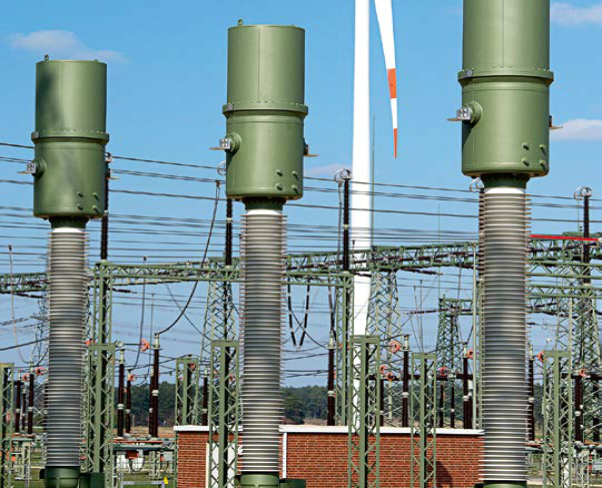
\includegraphics[width=0.98\columnwidth]{images/Messwandler.png}
    \end{center}
\end{minipage}
\hfill
\begin{minipage}[c]{0.48\columnwidth}
    \begin{center}
        \includegraphics[width=0.98\columnwidth]{images/Überspannungsableiter.png}
    \end{center}
\end{minipage}


\subsection{Schaltfelder Aufbau}

\begin{minipage}[c]{0.48\columnwidth}
    \subsubsection{Einfachsammelschiene}
\end{minipage}
\hfill
\begin{minipage}[c]{0.48\columnwidth}
    \subsubsection{Doppelsammelschiene}
\end{minipage}

\begin{minipage}[c]{0.48\columnwidth}
    \begin{itemize}
        \item übersichtliche und billige Lösung
    \end{itemize}
\end{minipage}
\hfill
\begin{minipage}[c]{0.48\columnwidth}
    \begin{itemize}
        \item ein Sammelschienenwechsel eines beliebigen Feldes jederzeit möglich
    \end{itemize}
\end{minipage}

\vspace{0.15cm}

\begin{minipage}[c]{0.48\columnwidth}
    \begin{center}
        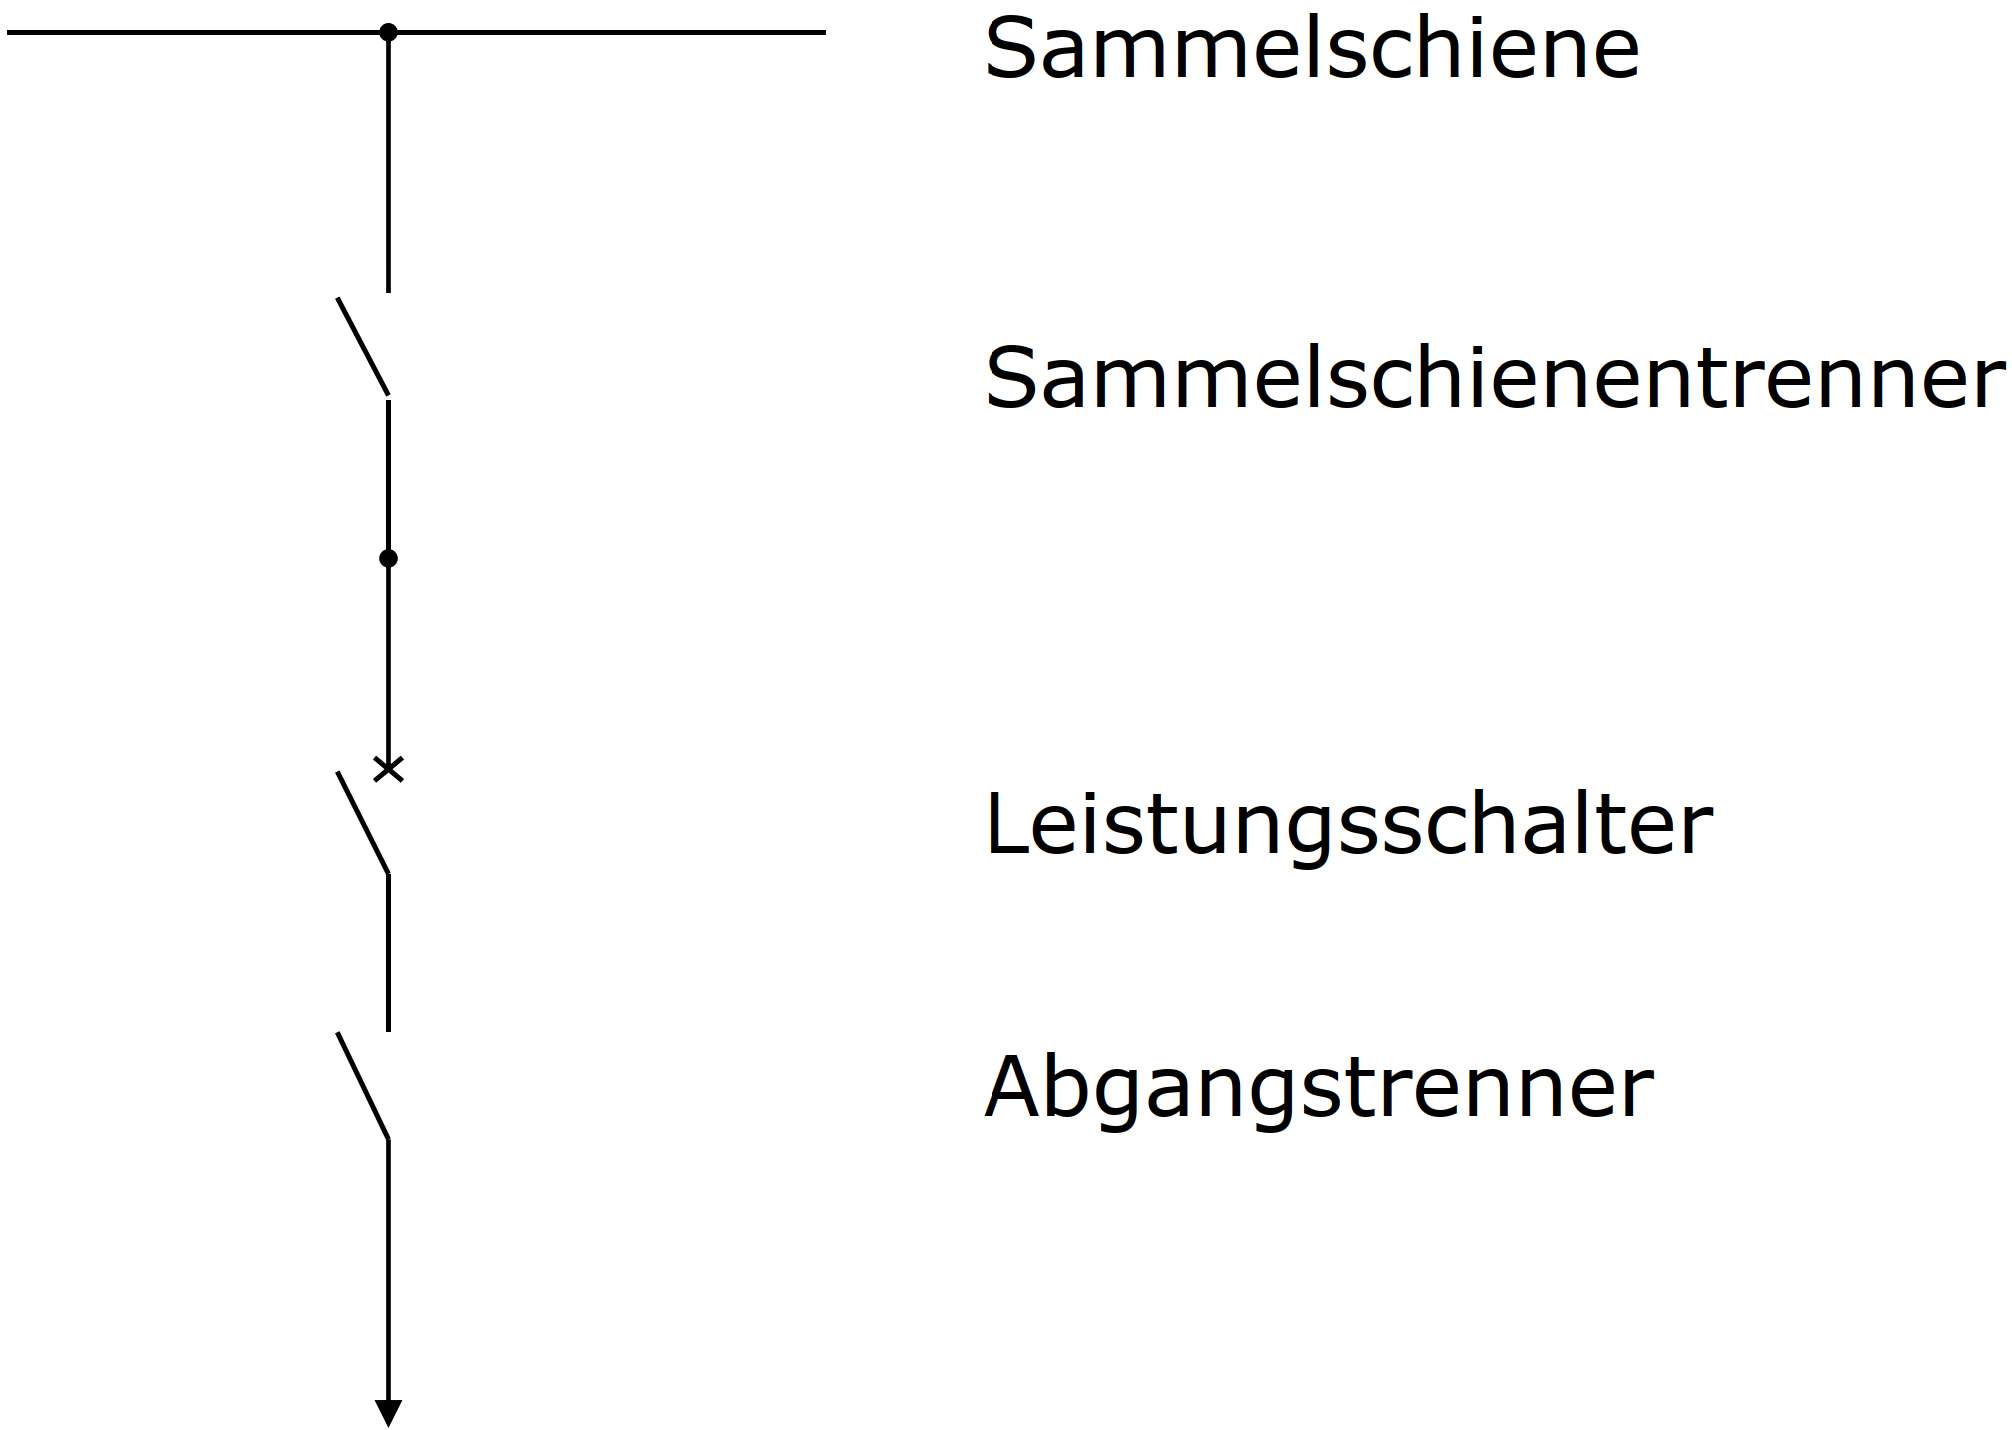
\includegraphics[width=0.98\columnwidth]{images/Einfachsammelschiene.png}
    \end{center}
\end{minipage}
\hfill
\begin{minipage}[c]{0.48\columnwidth}
    \begin{center}
        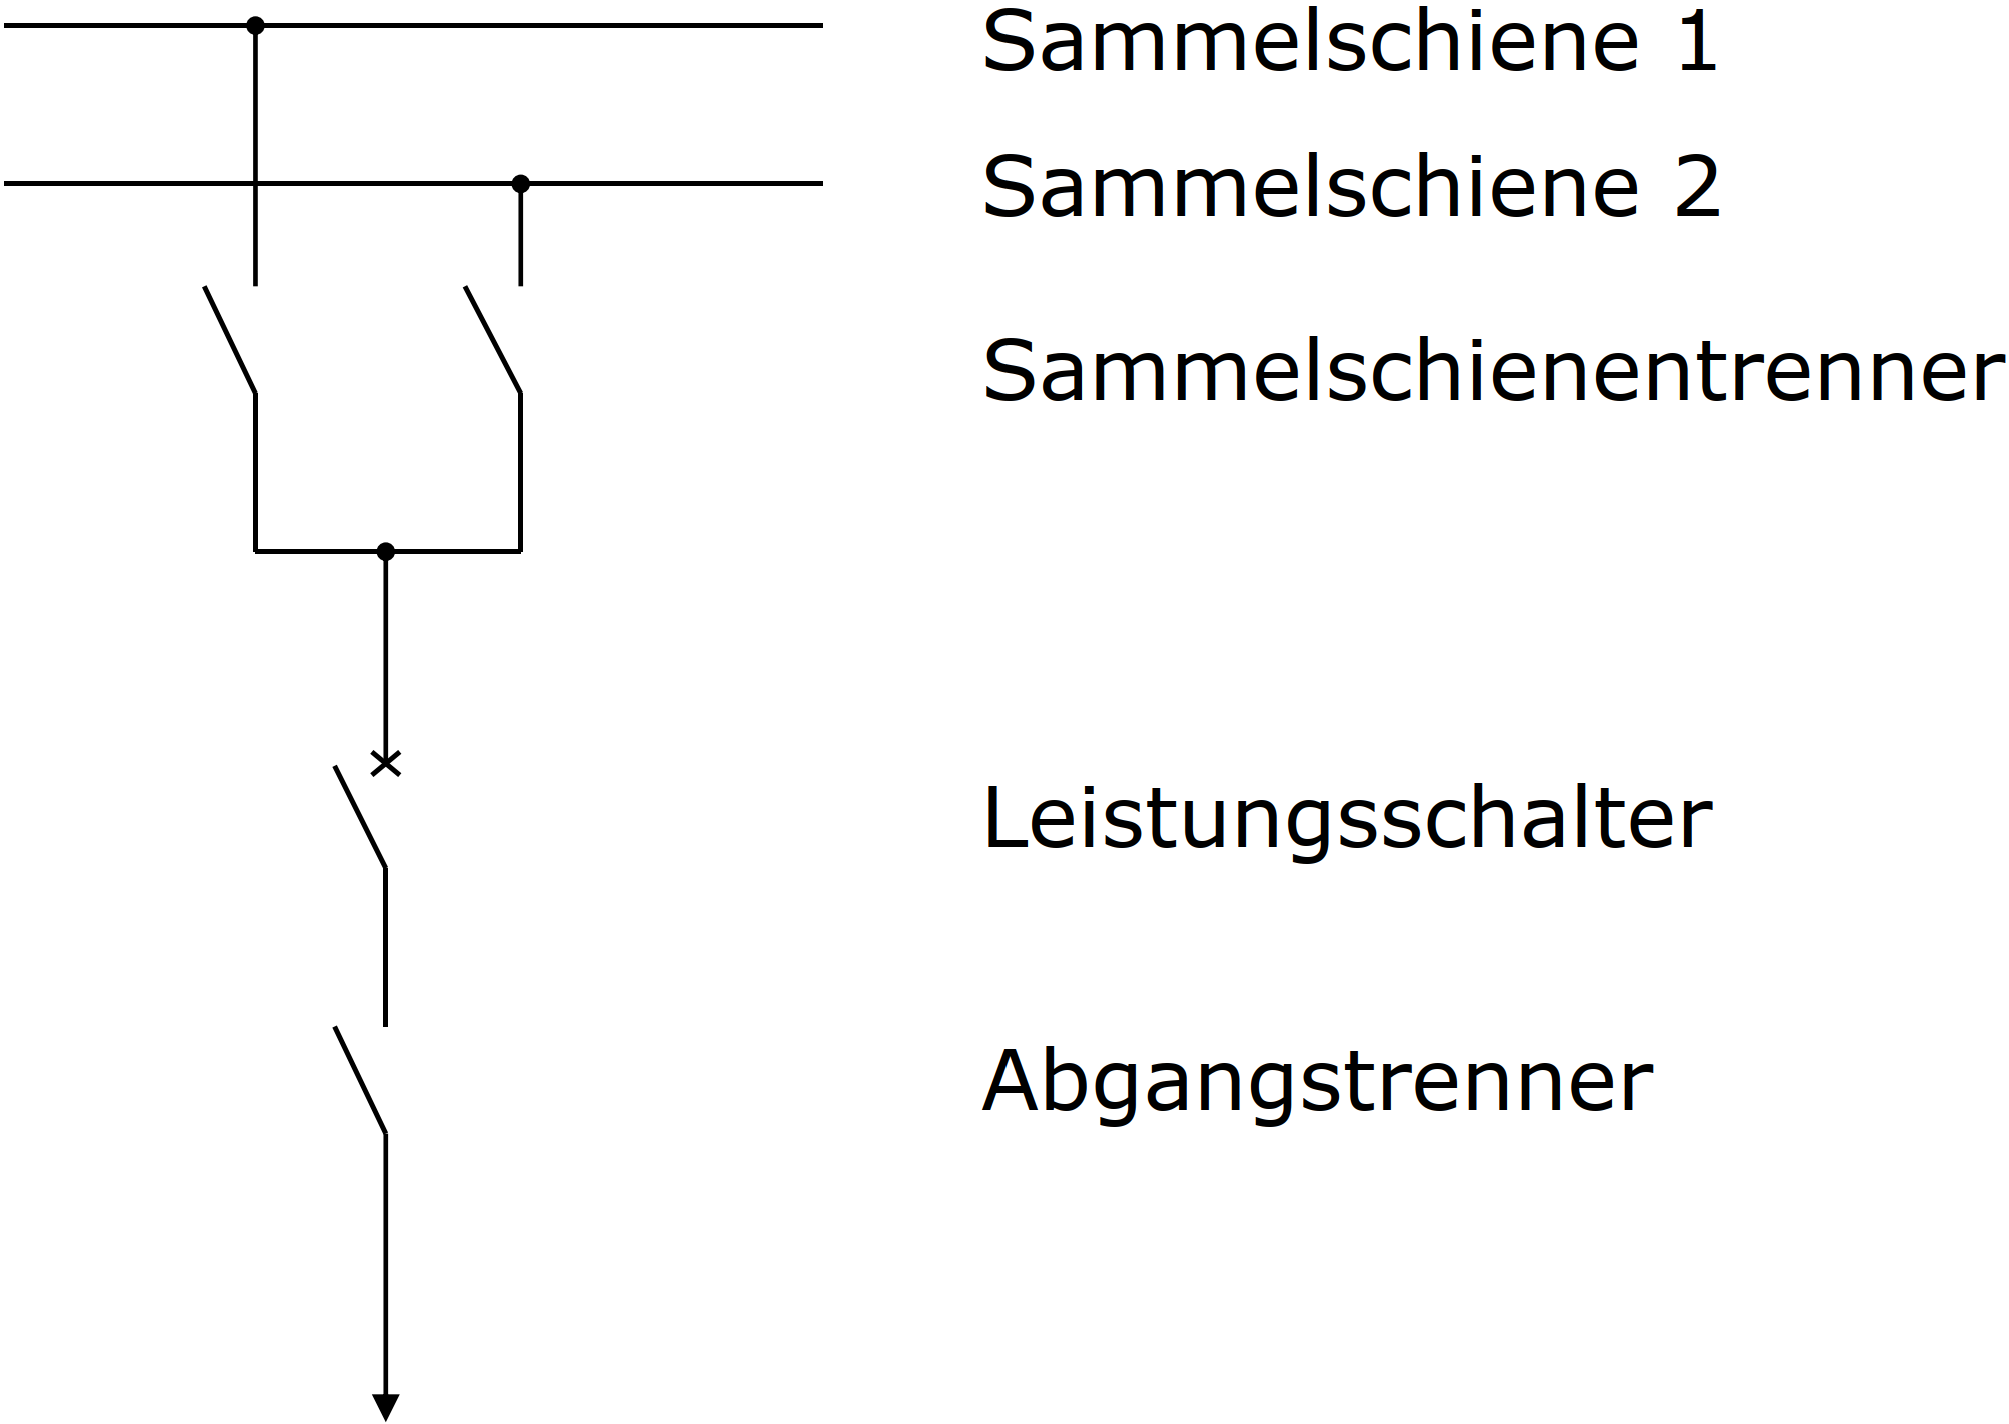
\includegraphics[width=0.98\columnwidth]{images/Doppelsammelschiene.png}
    \end{center}
\end{minipage}

\vspace{0.15cm}

\begin{minipage}[c]{0.48\columnwidth}
    \subsubsection{Sammelschienenkupplung}
\end{minipage}
\hfill
\begin{minipage}[c]{0.48\columnwidth}
    \subsubsection{Umgehungsschiene}
\end{minipage}

\begin{minipage}[c]{0.48\columnwidth}
    \begin{itemize}
        \item Ermöglicht die Parallelschaltung der beiden Sammelschienensysteme und damit den Sammelschienenwechsel des Feldes ohne Betriebsunterbruch
    \end{itemize}
\end{minipage}
\hfill
\begin{minipage}[c]{0.48\columnwidth}
    \begin{itemize}
        \item Bei dieser Schaltung ersetzt Reserveschalter den Kuppelschalter beim
        Sammelschienenwechsel
    \end{itemize}
\end{minipage}

\vspace{0.15cm}

\begin{minipage}[c]{0.48\columnwidth}
    \begin{center}
        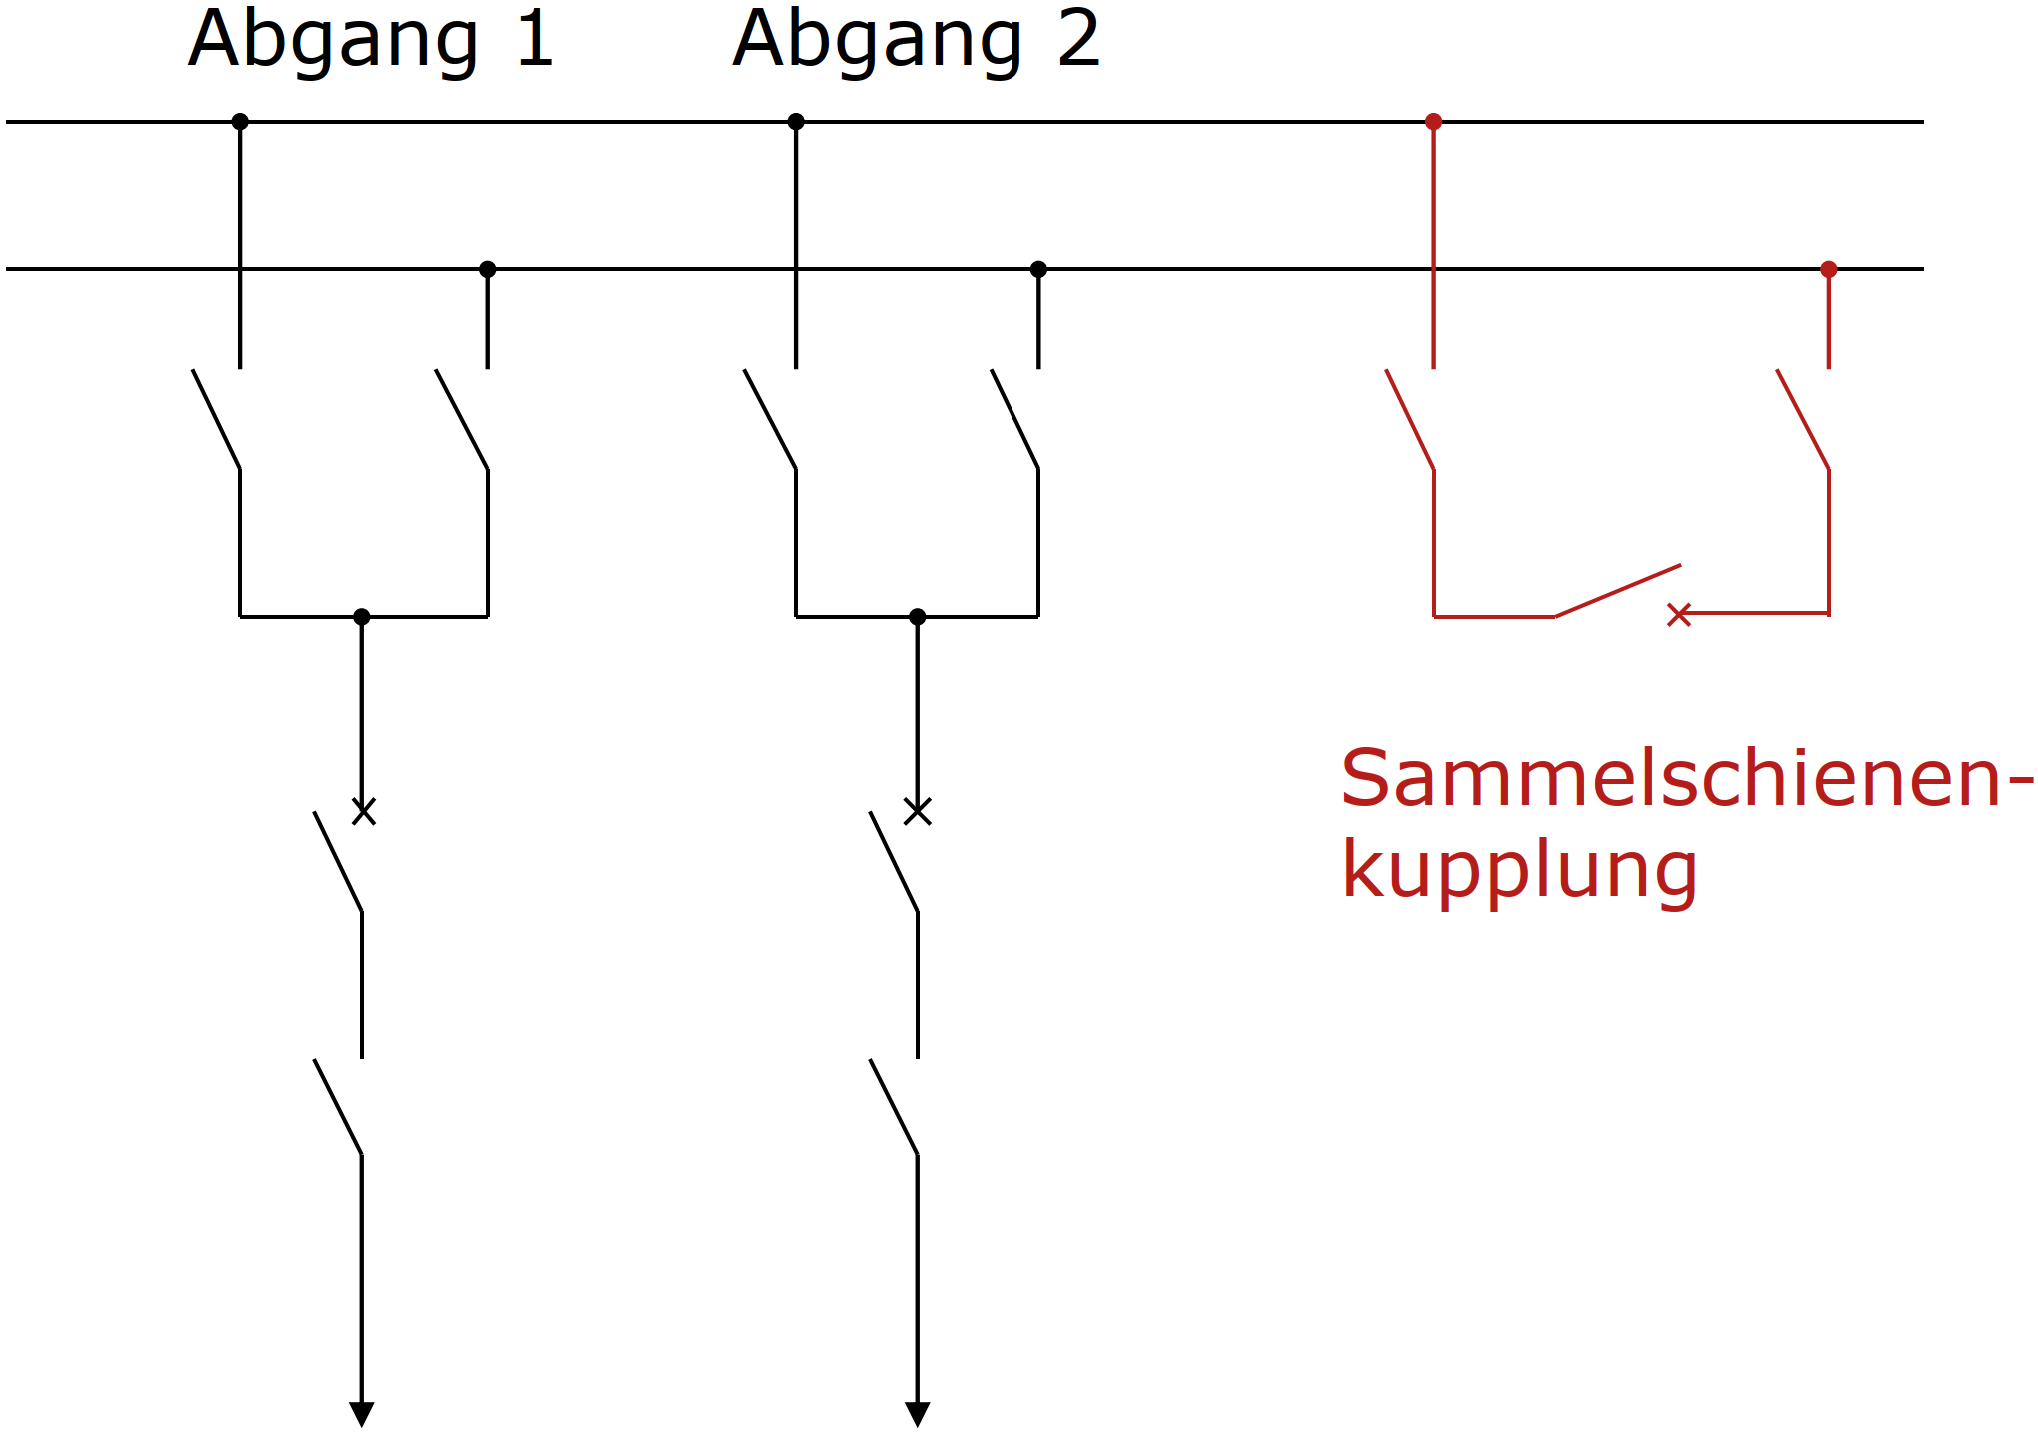
\includegraphics[width=0.98\columnwidth]{images/Sammelscheinenkupplung.png}
    \end{center}
\end{minipage}
\hfill
\begin{minipage}[c]{0.48\columnwidth}
    \begin{center}
        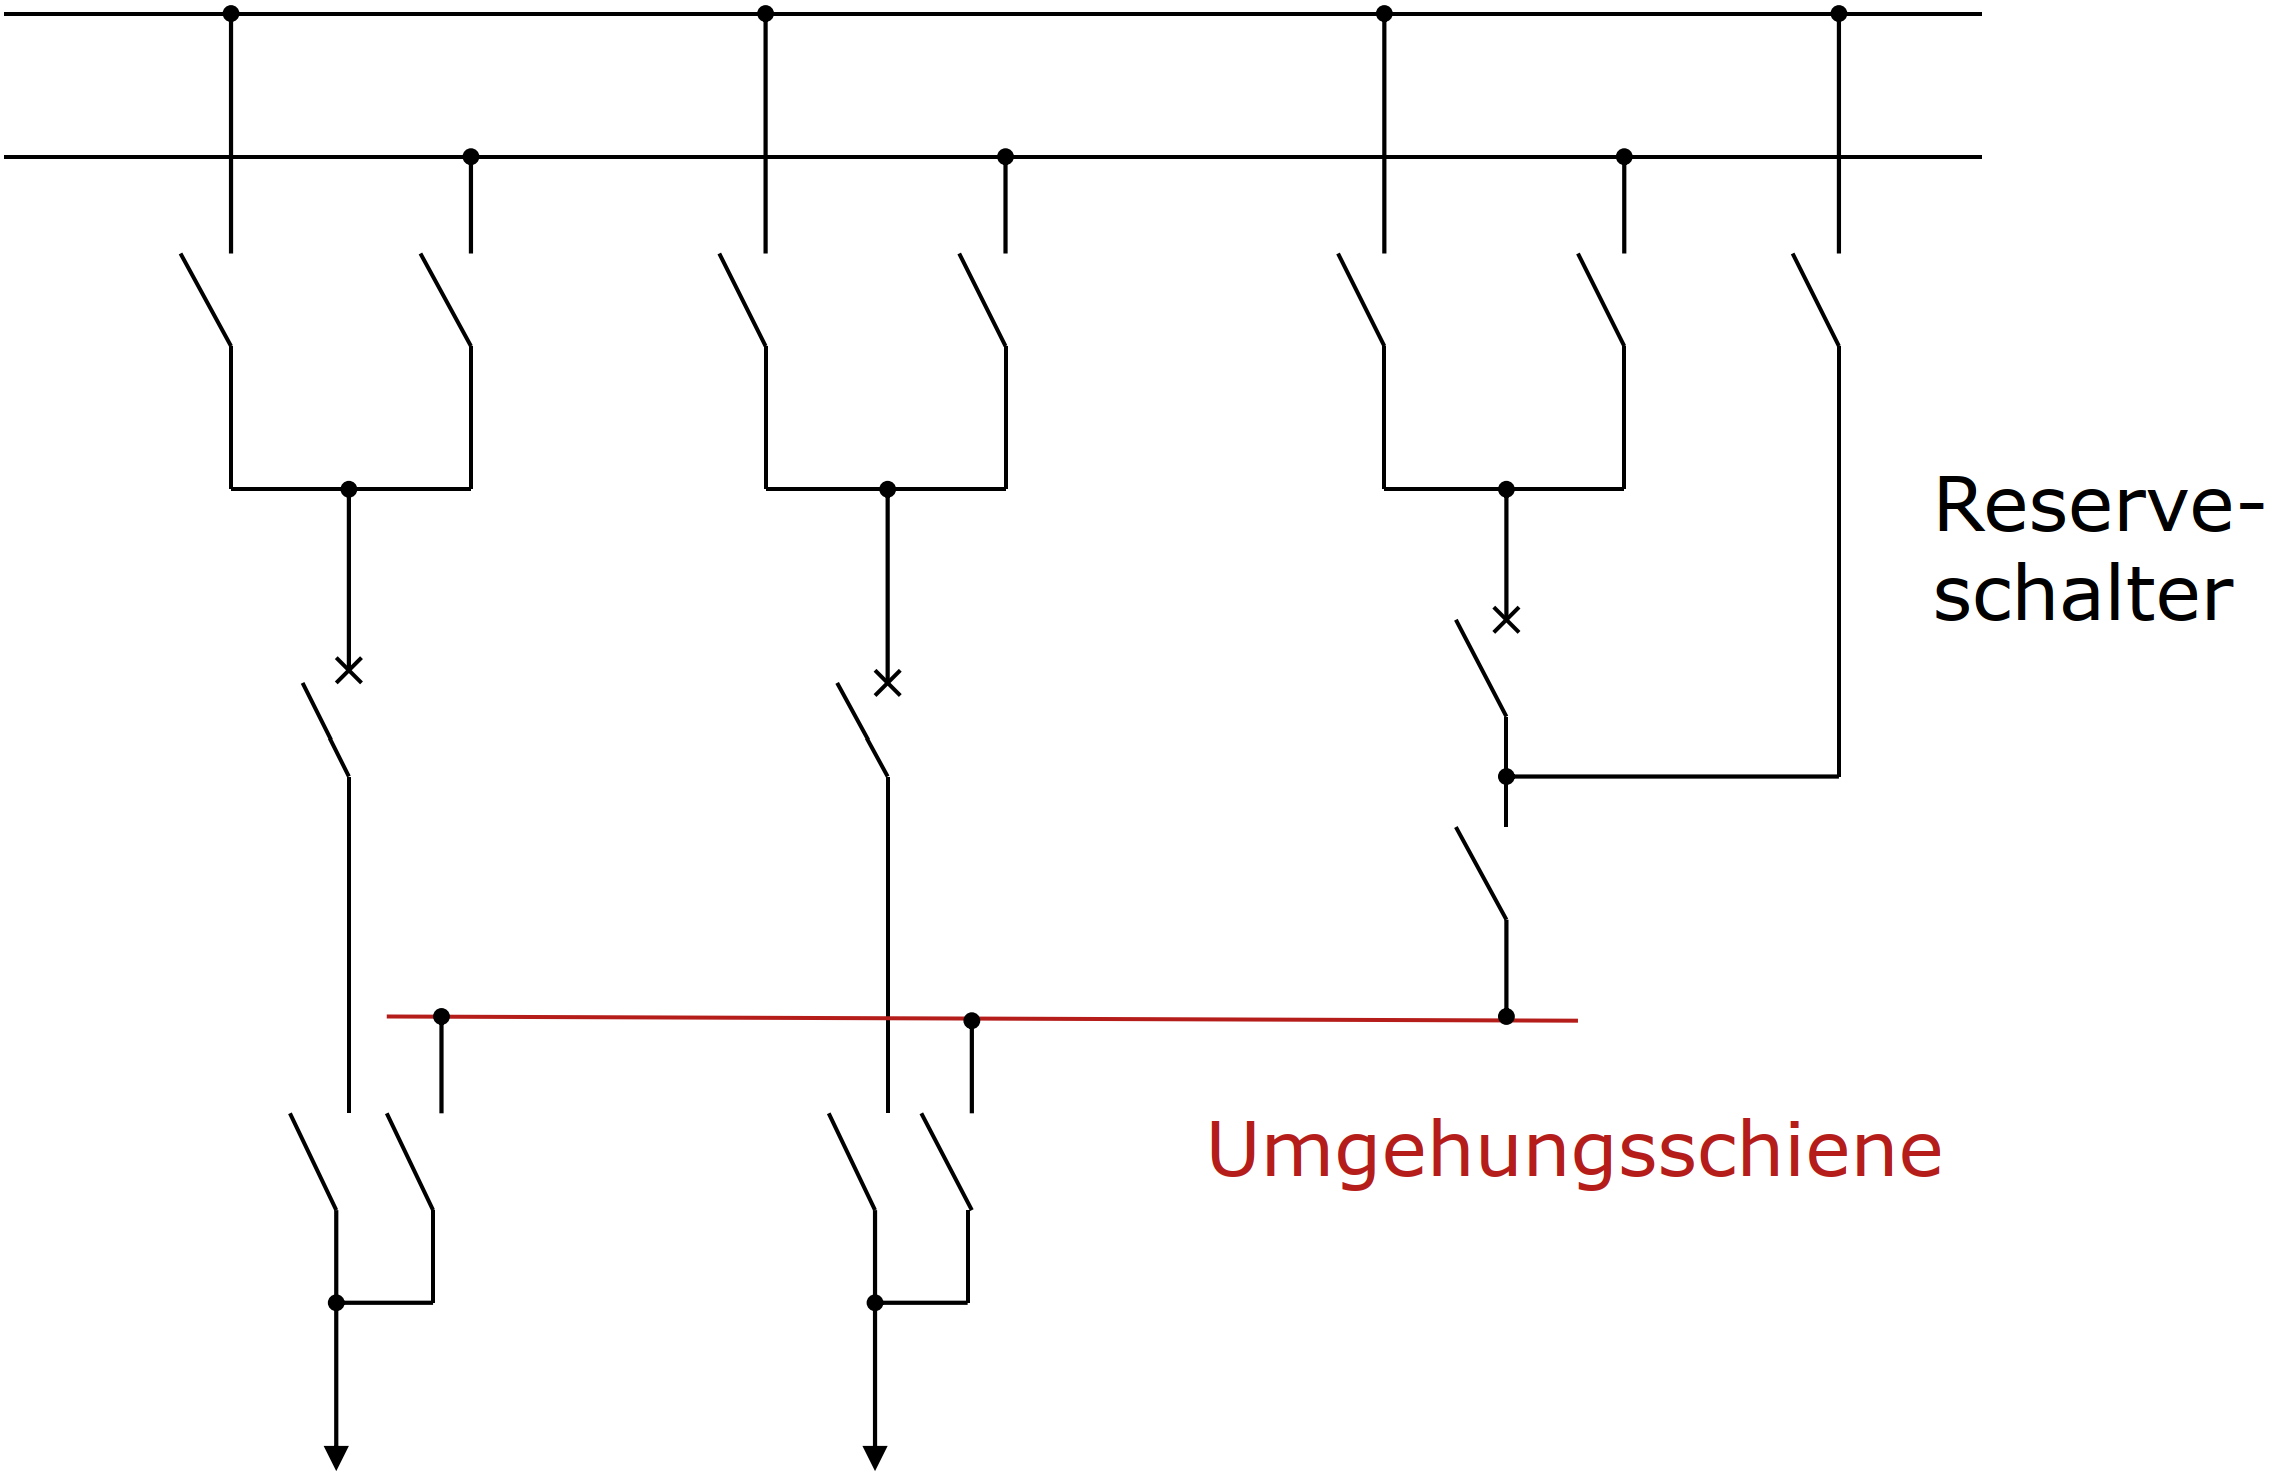
\includegraphics[width=0.98\columnwidth]{images/Umgehungsschiene.png}
    \end{center}
\end{minipage}

\subsection{Reglen beim Schalten (Reihenfolge)}

\subsubsection{Allgemein}
Es muss immer beidseitig Spannungsfrei sein, um ein Teil auszutauschen.\\
Es darf kein Strom fliessen.

\subsubsection{Ausschalten}
Beim Ausschalten werden Leistungsschalter zuerst geöffnet, dann Last- und Trennschalter
\subsubsection{Einschalten}
Beim Einschalten müssen zuerst Trennschalter, dann Lastschalter und zuletzt Leistungsschalter geschlossen werden






